\chapter{Background}
\label{sec:demo}
%
In this chapter bla bla
\todo{Describe Chapter}

% ====
% Autonomic computing
% ====
\section{Autonomic computing}
Autonomic computing is an architecture for computing systems to enable the ability to manage themselves in accordance to high level objectives configured by administrators \cite{Kephart2003VisionComputing}. 
These computing systems dynamically adapt to demands and conditions of the workload \cite{Kephart2003VisionComputing}.
An intelligent control-loop is responsible to collect all important details of the computing system and make decision according to the collected details. To automate the tasks, the intelligent control-loop is organized into four categories:

\begin{itemize}
\item \textbf{Self-configuring}
- Components in the environment have to adapt dynamically to system changes using policies. For example, deploying or removing new components.

\item \textbf{Self-healing}
- If system errors have being detected, the control-loop has to perform policy-based actions without disrupting the 
environment.

\item \textbf{Self-optimizing}
- The control-loop has to monitor the resources and should adapt to changes dynamically.

\item \textbf{Self-protecting}
- Detection and protection against threats.

\end{itemize}

 An autonomic computing environment consists of an autonomic manager, managed-resources and a knowledge-base.
 % As shown in figure ...
 
\subsection{Managed resources}
Managed resources are software or hardware components in the computing environment. For example, a managed resource 
can be a database, service, application, server or different entity. Each managed resource implements an interface to enable 
the autonomic manager to communicate with the managed resource. 

These interface are called touchpoints.

\subsection{Autonomic manager}
The autonomic manager implements an intelligent control-loop to collect system metrics from the managed resources and acts according to the collected details. It can only make adjustments within it`s own scope and uses policies to make decisions of what actions have to be
executed to accommodate the objectives.
To be self-managing, the autonomic manager has to implement the following four automated functions.

\begin{itemize}
\item \textbf{Monitor}
- The monitor function is responsible to collect the needed metrics from all managed resources and applies aggregation and filter
operations to the collected data. After that the function reports the metrics.

\item \textbf{Analyze}
- To determine if changes have to be made to the computing system, the collected data has to be analyzed.

\item \textbf{Plan}
- If changes have to be made, an appropriate change plan has to be generated. A change plan consists of actions that are needed to achieve the configured goals and objectives. The change plan needs to be forwarded to the execute function.

\item \textbf{Execute}
- The execute function applies all necessary changes to the computing system.

\end{itemize}

Multiple autonomic manager can exist in an autonomic computing environment to perform only certain parts. For example, 
there can be one autonomic manager which is responsible to monitor and analyze the system and another autonomic manager 
to plan and execute. To create a complete and closed control-loop, multiple autonomic manager can be composed together.


\section{Docker}


\section{Apache Spark}
Apache Spark is an open-source computing framework for parallel data processing on a large computer cluster. Spark manages the available resources and distributes computation tasks across a cluster to perform big-data processing operations at large scale \cite{Chambers2018Spark}. Before Spark was developed, Hadoop MapReduce \cite{Dean2010MapReduce} was the framework of choice for parallel operations on a computer cluster \cite{Zaharia2010Spark}. Spark accomplished to outperform Hadoop by 10x for iterative Machine Learning \cite{Zaharia2010Spark}. It is implemented in Scala\footnote{Scala programming language. https://www.scala-lang.org/}, a JVM-based language and provides a programming interface for Scala, Java\footnote{Java programming language. https://www.oracle.com/java/}, Python\footnote{Python programming language. https://www.python.org/} and R\footnote{R programming language. https://www.r-project.org/}. In addition, Spark includes an interactive SQL shell and libraries to implement Machine Learning and streaming applications \cite{Chambers2018Spark}.
It was developed in 2009 as the Spark research project at UC Berkeley and became an Apache Software Foundation project in 2013 \cite{Chambers2018Spark}. 

%  MASTER SLAVE 

\subsection{Spark programming model}

Spark provides resilient distributed datasets (RDDs) as the main abstractation for parallel operations \cite{Zaharia2010Spark}. Core types of Spark`s higher-level structured API are built on top of RDDs \cite{Chambers2018Spark} and will automatically be optimized by Spark`s Catalyst optimizer to run operations quick and efficient \cite{Hien2018Spark}.
\todo{Master-Slave Architektur + Bild}


\paragraph{Resilient distributed datasets:}
% What are RDDs
Resilient distributed datasets are fault-tolerant, parallel data structures to enable data sharing across cluster applications \cite{Zaharia2012RDDs}. They allow to express different cluster programming models like MapReduce, SQL and batched stream processing \cite{Zaharia2012RDDs}. RDDs have been implemented in Spark and serve as the underlying data structure for higher level APIs (Spark structured API) \cite{Zaharia2012RDDs}.
% How can RDDs be used in applications    !! HIER MAL BEISPIEL WIE IN RDD ERZEUGT WIRD
RDD`s are a immutable, partitioned collection of records and can only be initiated through transformations (e.g. map, filter) on data or other RDD`s.
% What are the advantages of RDDs    !!! HIER NOCHMAL BEISPIEL WIE DAS AUSSEHEN KANN
An advantage of RDDs is, that they can be recovered through lineage. Lost partitions of an RDD can be recomputed from other RDDs in parallel on different nodes \cite{Zaharia2012RDDs}. 
% Better use structured API
RDDs are lower level APIs and should only be used in applications if custom data partitioning is needed \cite{Chambers2018Spark}. It is recommended to use Sparks structured API objects instead. Optimizations for RDDs have to be implemented manually while Spark automatically optimize the execution for structured API operations \cite{Chambers2018Spark}.


\paragraph{Spark structured API:}
% What is the structured API
Spark provides high level structured APIs for manipulating all kinds of data. The three distributed core types are Datasets, DataFrames and SQL Tables and Views \cite{Chambers2018Spark}.
% About DataFrames, Datasets and SQL
Datasets and DataFrames are immutable, lazy evaluated collections that provide execution plans for operations \cite{Chambers2018Spark}. SQL Tables and Views work the same way as DataFrames, except that SQL is used as the interface instead of using the DataFrame programming interface \cite{Chambers2018Spark}.
% Differences between Datasets ad Dataframes
Datasets use JVM types and are therefore only available for JVM based languages. DataFrames are Datasets of type Row, which is the Spark internal optimized format for computations. This has advantages over JVM types which comes with garbage collection and object instantiation \cite{Chambers2018Spark}.


\paragraph{Spark Catalyst:}
% What is the Catalyst optimizer
Spark also provides a query optimizer engine called Spark Catalyst. \Fig{fig:spark_catalyst_process} illustrates how the Spark Catalyst optimizer automatically optimizes Spark applications to run quickly and efficient.
% Short How
Before executing the user`s code, the Catalyst optimizer translates the data-processing logic into a logical plan and optimizes the plan using heuristics \cite{Hien2018Spark}. After that, the Catalyst optimizer converts the logical plan into a physical plan to create code that can be executed \cite{Hien2018Spark}.


% What are logical plans
Logical plans get created from a DataFrame or a SQL query. A logical plan represents the data-processing logic as a tree of operators and expressions where the Catalyst optimizer can apply sets of rule-based and cost-based optimizations \cite{Hien2018Spark}.
For example, the Catalyst can position a filter transformation in front of a join operation \cite{Hien2018Spark}.

% What are physical plans
From the logical plan, the Catalyst optimizer creates one ore more physical plans which consist of RDD operations \cite{Chambers2018Spark}. The cheapest physical will be generated into Java bytecode for execution across the cluster \cite{Hien2018Spark}.

% Spark Catalyst figure
\begin{figure}[h]%
\centering
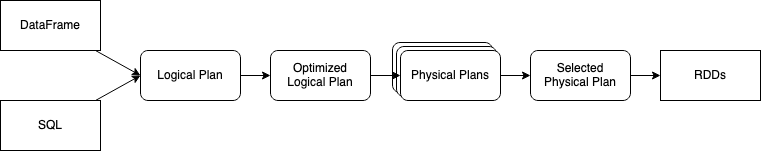
\includegraphics[scale=0.5]{images/03_background/spark_catalyst}%
\caption{Optimization process of the Spark Catalyst - Source: Authors own model, based on \cite{Hien2018Spark}.}%
\label{fig:spark_catalyst_process}%
\end{figure}
\todo{Bild nochmal machen mit abstand	+ QUELLE anpassen}


\subsection{Spark application architecture}

\begin{figure}[h]%
\centering
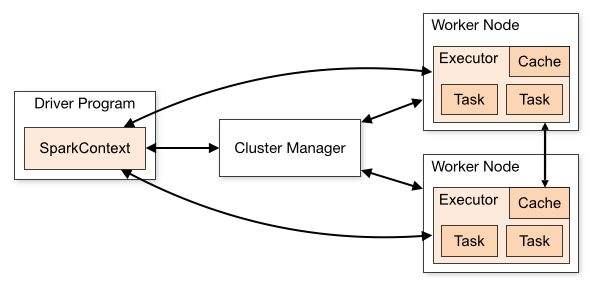
\includegraphics[scale=0.5]{images/03_background/cluster_overview}%
\caption{Overview of a Spark cluster architecture - Source: Authors own model, based on \cite{Apache2020Spark}.}%
\label{fig:spark_cluster_overview}%
\end{figure}

\todo{Lieber Doch Master/Slave ???. Was ist mit dem CLuster-Manager}
% Explain image
\Fig{fig:spark_cluster_overview} illustrates the main architecture of a Spark cluster. The architecture follows the master-worker model where the Spark driver is the master and the Spark executors are the worker \cite{Hien2018Spark}.
\todo{Nicht ganz richtig, Master und Worker sind machines und driver und executor sind prozesse}

\paragraph{Spark driver:}
The Spark driver is a JVM process on a physical machine and responsible to maintain the execution of a Spark application \cite{Chambers2018Spark}. It coordinates the application tasks onto each available executor \cite{Hien2018Spark}. To get launch executors and get physical resources, the Spark driver interacts with the cluster manager \cite{Chambers2018Spark, Hien2018Spark}.


\paragraph{Spark Executor:}
A Spark executor performs the tasks given by the Spark driver \cite{Chambers2018Spark}. It runs as a JVM process and runs until the Spark application finishes \cite{Hien2018Spark}. After the executor finishes, it reports back to the Spark driver \cite{Chambers2018Spark}. Each task will be performed on a separate CPU core to enable parallel processing  \cite{Hien2018Spark}.


\paragraph{Cluster manager:}
The cluster manager is an external service that orchestrates the work between the machines in the cluster \cite{Hien2018Spark, Apache2020Spark}. The cluster manager knows about the resources of each worker and decides on which machine the Spark driver process and the executor processes run \cite{Hien2018Spark, Chambers2018Spark}.
% Different cluster types
Spark supports different services that can run as the cluster manager: Standalone, Apache Mesos\footnote{Apache Mesos. https://mesos.apache.org/}, Hadoop YARN\cite{Murthy2013Yarn} and Kubernetes\footnote{Kubernetes. https://kubernetes.io/} \cite{Apache2020Spark}.
% What is standalone
\todo{Explain standalone}
% Explain different cluster deploy modes
The cluster manager provides three different deploy modes for acquiring resources in the cluster.
\begin{itemize}
\item Cluster mode
\item Client mode
\item Local mode
\end{itemize}

% Cluster mode
To run an application in cluster mode, the user has to submit a precompiled JAR, python script or R script to the cluster manager \cite{Chambers2018Spark}. After that, the cluster manager starts the driver process and executor processes exclusively for the Spark application on machines inside the cluster \cite{Chambers2018Spark, Hien2018Spark}.
\begin{figure}[h]%
\centering
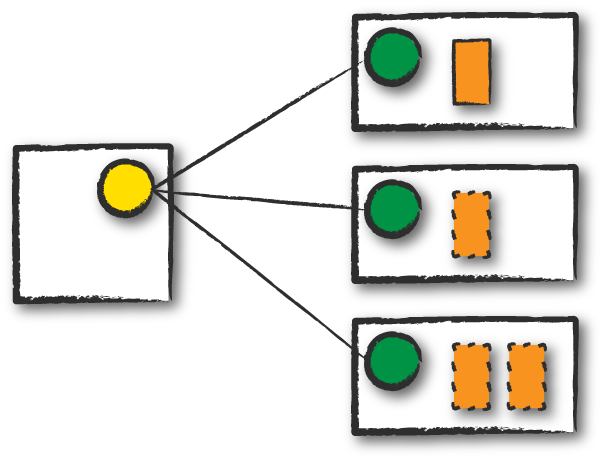
\includegraphics[scale=0.5]{images/03_background/cluster_mode}%
\caption{Spark`s cluster mode - Source: Authors own model, based on \cite{Chambers2018Spark}.}%
\label{fig:spark_cluster_mode}%
\end{figure}

% Client mode
The difference between the client mode and the cluster mode is that, the driver process runs on the client machine outside of the Spark cluster \cite{Chambers2018Spark}.
\begin{figure}[h]%
\centering
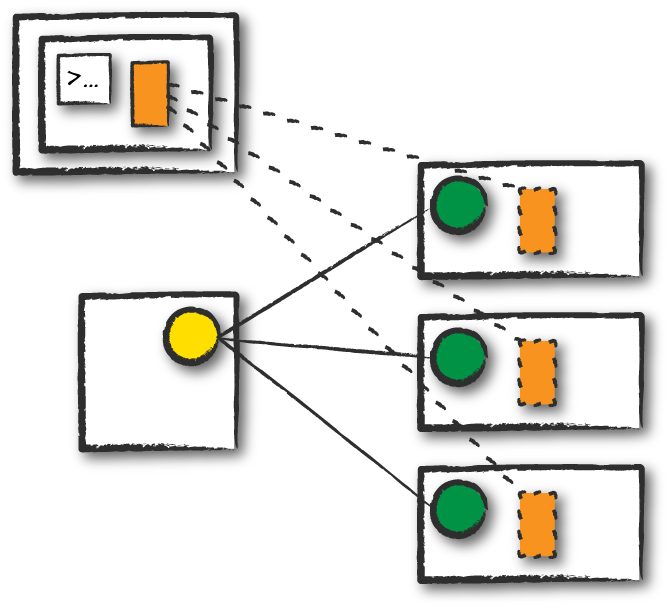
\includegraphics[scale=0.5]{images/03_background/client_mode}%
\caption{Spark`s client mode - Source: Authors own model, based on \cite{Chambers2018Spark}.}%
\label{fig:spark_client_mode}%
\end{figure}

% Local mode
The local mode starts a Spark application on a single computer \cite{Chambers2018Spark}. It is not recommended to use the local mode in production, instead it should be used for testing Spark applications or learning the Spark framework \cite{Chambers2018Spark}.


\subsection{Spark application implementation}
% Short intro
The concept of a Spark application consists of calling transformations and actions. A transformation creates a DataFrame or a Dataset, the logical data structures of a Spark application. The computation of a Spark application gets processed when an action gets called in the application. The transformations of a Spark application build up a directed acyclic graph (DAG) of instructions. By calling an action, the DAG will break down into stages and tasks to create a single job for execution \cite{Chambers2018Spark}.
% Show example application
\begin{lstlisting}[frame=single, caption=Example of a Python 3 Spark application, captionpos=b]
# Initialize a SparkSession
sparkSession = SparkSession\
    .builder\
    .getOrCreate()

# Create a dataframe with a transformation
dataframe = sparkSession.range(1, 1000)
# Apply another transformation
dataframe = dataframe.filter(dataframe.id % 2 == 0)
# Call an action
count = dataframe.count()
\end{lstlisting}
% Explain a spark application on top of an example
LISTING XYZ demonstrates how a Spark application can be implemented. At first a SparkSession gets initialized. Each Spark application must include a SparkSession to BLA BLA \cite{Chambers2018Spark}. After that, a DataFrame gets created with the range transformation to include each number from 1 to 1000 in the DataFrame. Next, a filter transformation is applied on the DataFrame to sort out any odd number. At the end, the number of rows gets saved in a variable with the count action.


\subsection{spark-submit}


\section{Prometheus}


\section{NVIDIA RAPIDS}


\section{Gitlab CI/CD}


\section{K-MEANS}


\section{Naive Bayes Classifier}


\section{Scaling heat}


\section{KHP}